\subsubsection{Actinemys --- Western Pond Turtles}
\begin{center}
\begin{longtabu} to \textwidth {| | p{3.5cm} | X | |}

	\hline
	Taxonomy/Ancestry &
	emydinae subfamily. originally, its single species was considered to be part of \emph{Clemmys}.
	
	\begin{center} \includegraphics[scale=0.5]{testudines/emydidae/actinemys/tax} \end{center}
	 \\
	\hline
	Size & 
	up to 20 cm (8 in) in carapace length.
	\\
	\hline
	Color &
	dorsal color --- dark brown, dull olive.
	
	yellow plastron w/ dark blotches in acute center.
	 \\
	\hline
	Anatomy &
	\begin{itemize}[noitemsep]
		\item low, broad carapace which is widest behind the middle. in adults, it is smooth, containing no keels* or serrations.
		\item grow slowly in wild --- age at 1st reproduction may be 10-12 yrs 
		\item may survive $>$50 yrs in wild
	\end{itemize}
	 \\
	\hline
	Dimorphism & 
	males have light/pale-yellow throat.
	\\
	\hline
	Behavior & 
	frequently bask, and can be encouraged to bask on artificial surfaces for easier study.
	\\
	\hline
	Habitat & 
	\begin{itemize}[noitemsep]
		\item occur in both permanent and intermittent waters --- marshes, streams, rivers, ponds, lakes
		\item favor habitats w/ many emergent logs/boulders to bask
		\item bask on top of aquatic vegetation, and are consequently often overlooked in the environment
		\item terrestrial habitat also important b/c they can spend up to 200 days outside of water when aquatic habitat dries (intermittent ponds), and many overwinter outside the water
	\end{itemize}
	\\
	\hline
	Distribution & 
	originally, the western pond turtle ranged from northern Baja California, Mexico, north to Puget Sound, Washington. however, as of 2007, they are rare/absent in Puget Sound. they have a disjunct distribution in most of Northwest, isolated populations in southern Washington, and may be locally common in some streams, rivers, and ponds in southern Oregon. they also occur in Uvas Canyon area, Santa Cruz Mts, California, in Northbay, lakes such as Fountaingrove lake. they range up to 305 m (1,001 ft) in Washington, up to 915 m (3,002 ft) in Oregon.
	
	\begin{center} \includegraphics[scale=0.8]{testudines/emydidae/actinemys/range} \end{center}
	\\
	\hline
	Feeding Ecology & 
	omnivorous, they often eat:
	\begin{itemize}[noitemsep]
		\item insects, crayfish, aquatic vertebrates
		\item fish, tadpoles, frogs, carrion rarely
		\item filamentous algae, lily pads, tule, cattail roots
	\end{itemize}
	generally, they are well protected due to their shells, but are threatened by predators such as raccoons, otters, ospreys, coyotes. hatchlings may be preyed on by weasels, bullfrogs, large fish.
	\\
	\hline
	Reproductive Biology & 
	\begin{itemize}
		\item 5-13 eggs per clutch in annual or biannual egg-layings
		\item may travel some distance from water for egg-laying, as much as 0.8 km (1/2 mi) away from and up to 90 m (300 ft) above nearest source of water. however, most nests are within 90 m (300 ft) of water 
		\item the female leaves water in evening, selects nest site in open area of sand or hardpan facing southwards
		\item flask-shaped nest w/ abt 5 cm (2 in) opening; the female covers nest w/ soil/adjacent low vegetation
		\item the vast majority of hatchlings overwinter in the nest
		\item winter rains may be necessary to loosen hardpan soil where nest is
		\item young first appear in spring following egg deposition
	\end{itemize}
	\\
	\hline
	Ecological Role &
	
	\\
	\hline
	Conservation Status & 
	listed as VU due to human threat, they face extinction due to the removal of ponds, wetlands, and the contamination of water sources.
	\\
	\hline
\end{longtabu}
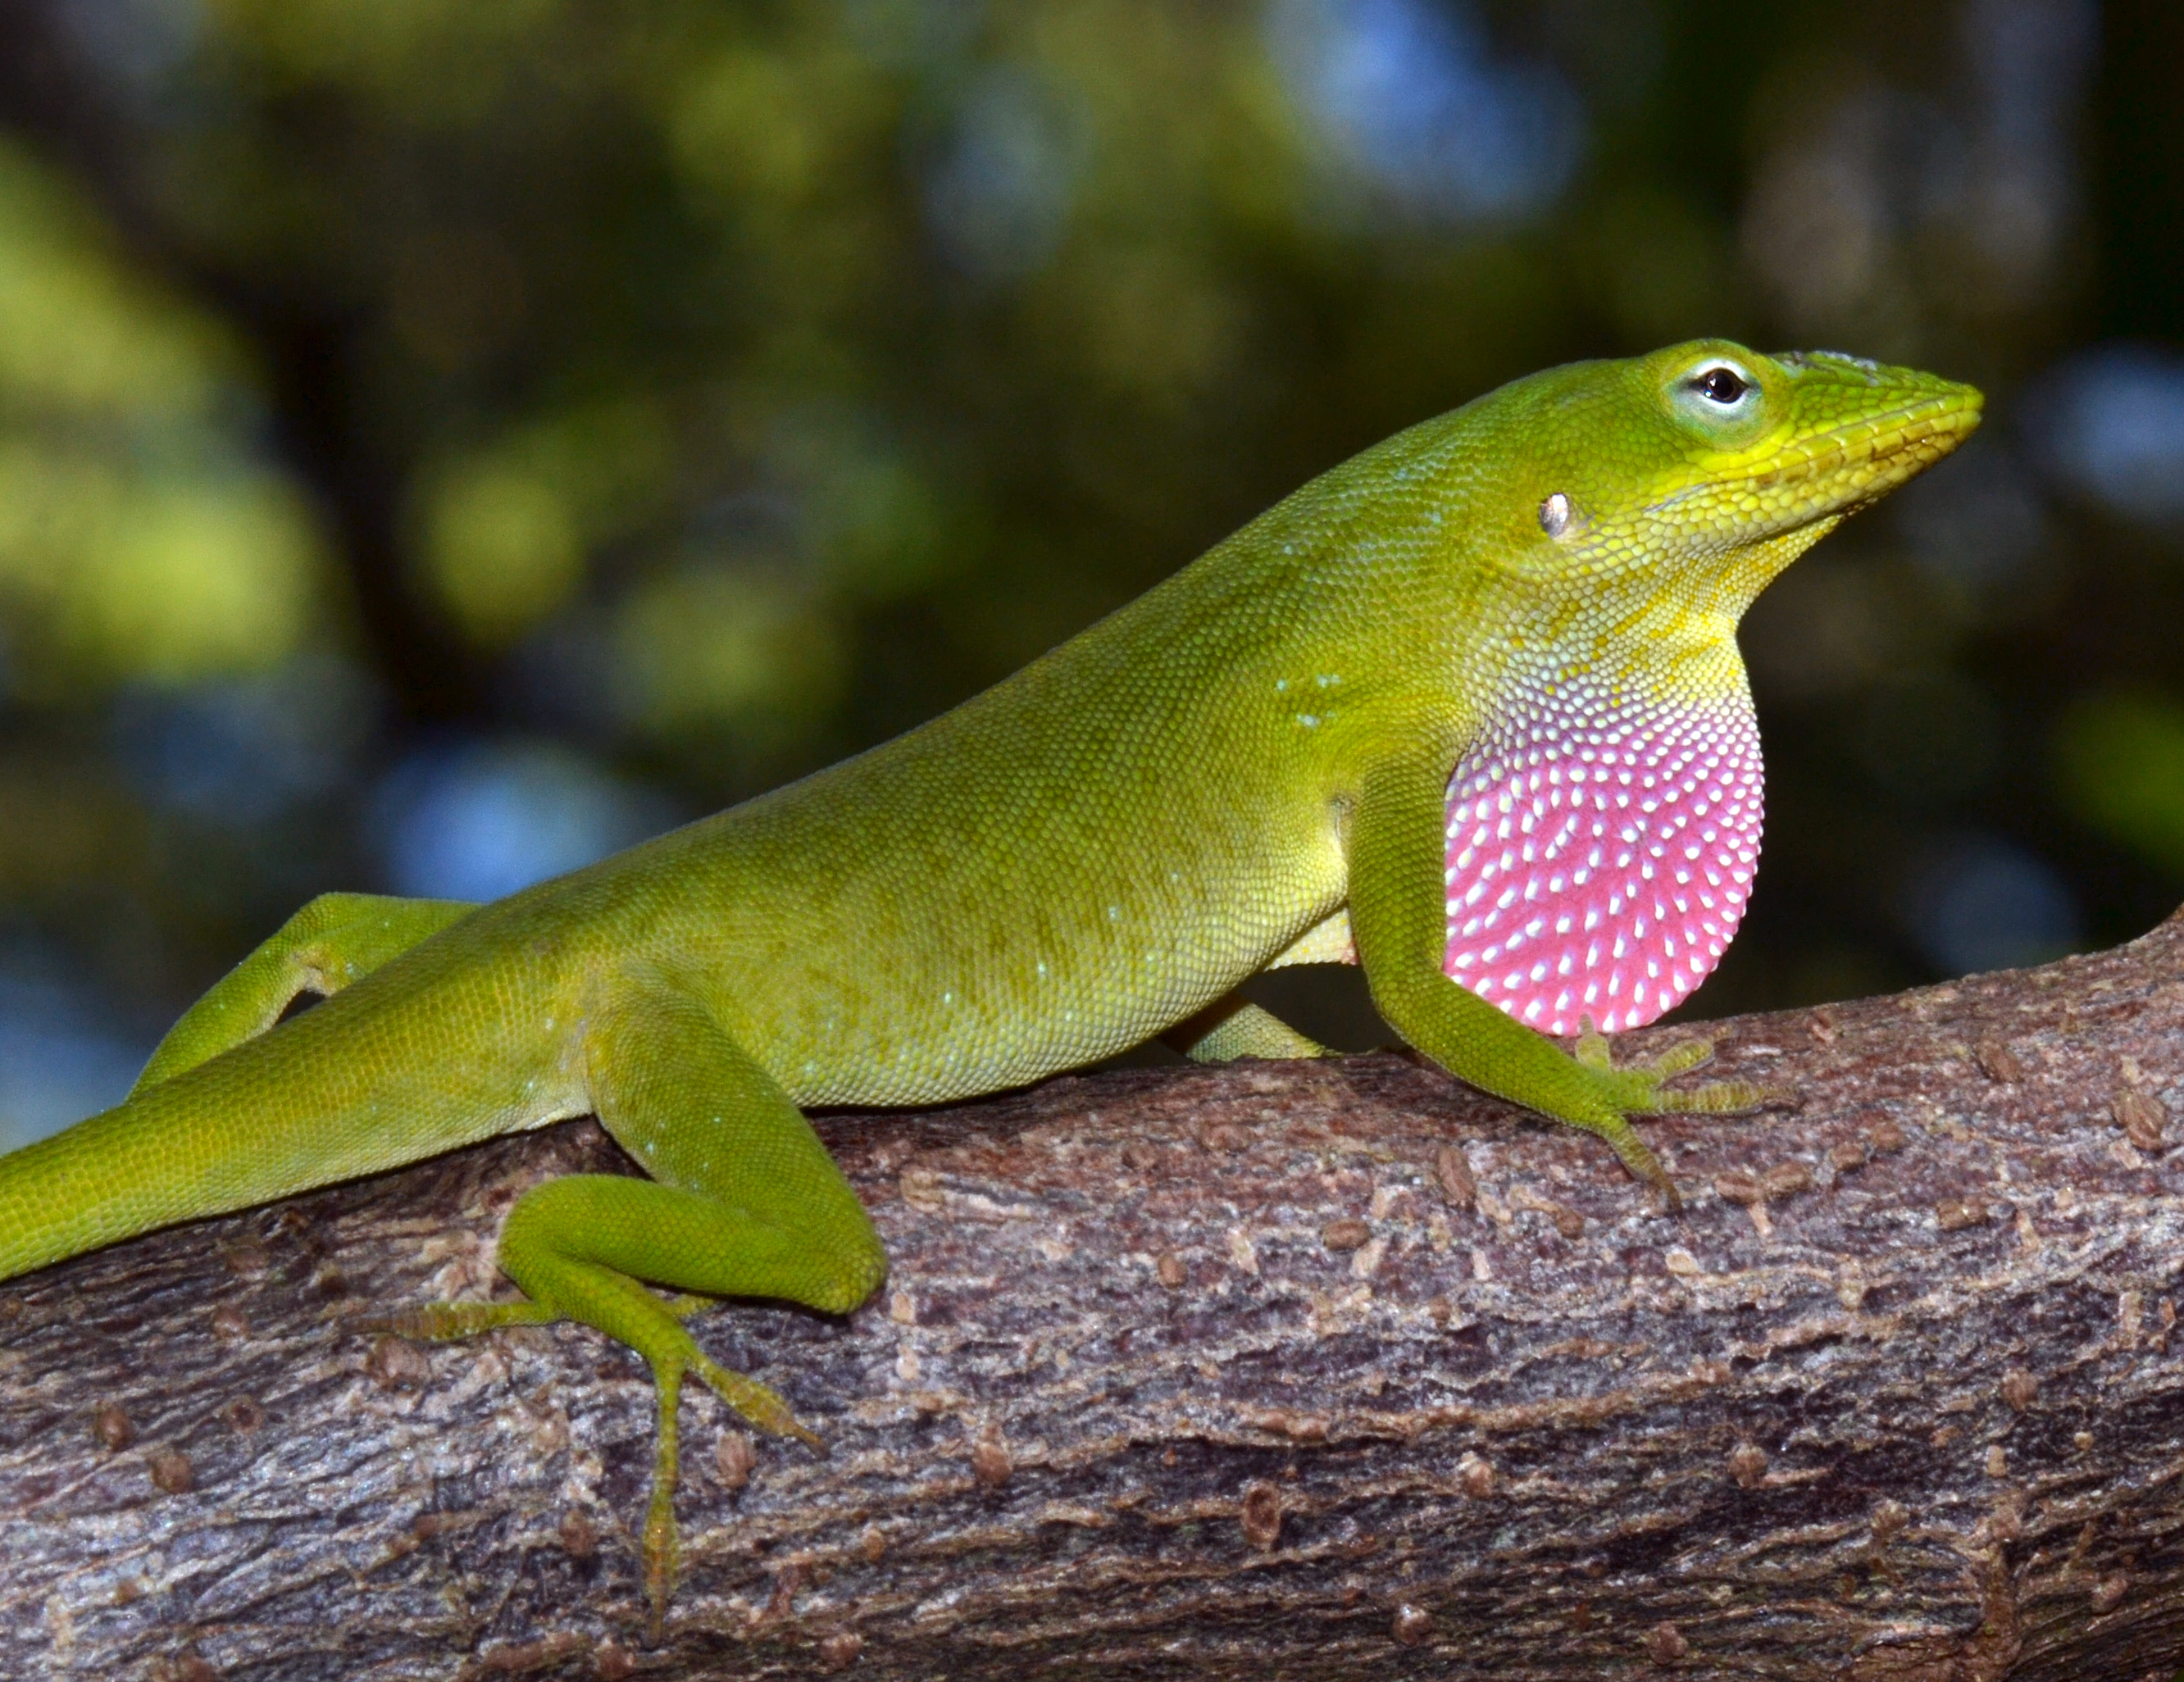
\includegraphics[scale=0.5]{testudines/emydidae/actinemys/1}
\includegraphics[scale=0.25]{testudines/emydidae/actinemys/3}
\end{center}